%% ----------------------------------------------------------------
%% Thesis.tex -- MAIN FILE (the one that you compile with LaTeX)
%% ---------------------------------------------------------------- 

% Set up the document
\documentclass[a4paper, 11pt, oneside]{uet_thesis}  % Use the "Thesis" style, based on the ECS Thesis style by Steve Gunn
\graphicspath{{Figures/}}  % Location of the graphics files (set up for graphics to be in PDF format)

% Include any extra LaTeX packages required
\usepackage[square, numbers, comma, sort&compress]{natbib}  % Use the "Natbib" style for the references in the Bibliography

\usepackage{verbatim}  % Needed for the "comment" environment to make LaTeX comments

\usepackage{vector}  % Allows "\bvec{}" and "\buvec{}" for "blackboard" style bold vectors in maths

\usepackage{url}
\usepackage{natbib}
\usepackage{amsmath}

\hypersetup{urlcolor=blue, colorlinks=true}  % Colours hyperlinks in blue, but this can be distracting if there are many links.

% remove the unnecessary spacing before and after the headings/subheadings
\usepackage[compact]{titlesec}
\titlespacing{\section}{0pt}{*0}{*0}
\titlespacing{\subsection}{0pt}{*0}{*0}
\titlespacing{\subsubsection}{0pt}{*0}{*0}

\setlength{\parskip}{6pt}
%\setlength{\parsep}{0pt}
%\setlength{\headsep}{0pt}
%\setlength{\topskip}{0pt}

%% ----------------------------------------------------------------
\begin{document}
\frontmatter	  % Begin Roman style (i, ii, iii, iv...) page numbering

% Set up the Title Page
\title  {A Simple Sampler using 555 Timerr}
\session {2017 -- 2021}
\advisor {Ma'am Aqsa}
\authors {
Usman IlamDin \\
}

\addresses  {\deptname \\ \univname}  % Do not change this here, instead these must be set in the "Thesis.cls" file, please look through it instead
\date       {\today}
\subject    {}
\keywords   {}

\maketitle
%% ----------------------------------------------------------------

\setstretch{1.3}  % It is better to have smaller font and larger line spacing than the other way round

% Define the page headers using the FancyHdr package and set up for one-sided printing
\fancyhead{}  % Clears all page headers and footers
\rhead{\thepage}  % Sets the right side header to show the page number
\lhead{}  % Clears the left side page header

\pagestyle{fancy}  % Finally, use the "fancy" page style to implement the FancyHdr headers


%% Select only one of the certification pages  
%\CertificationMSc{}
%\CertificationBSc{}
%\clearpage  % Certification ended, now start a new page



%\setstretch{1.3}  % Reset the line-spacing to 1.3 for body text (if it has changed)

% The Acknowledgements page, for thanking everyone
%\acknowledgements{
%\addtocontents{toc}{\vspace{1em}}  % Add a gap in the Contents, for aesthetics

%The acknowledgements and the people to thank go here, don't forget to include your project advisor\ldots

%}
%\clearpage  % End of the Acknowledgements
%% ----------------------------------------------------------------
\lhead{\emph{Contents}}  % Set the left side page header to "Contents"
\tableofcontents  % Write out the Table of Contents

%% ----------------------------------------------------------------
\lhead{\emph{List of Figures}}  % Set the left side page header to "List if Figures"
\listoffigures  % Write out the List of Figures

%% ----------------------------------------------------------------
%% ----------------------------------------------------------------
% End of the pre-able, contents and lists of things
% Begin the Dedication page
%\setstretch{1.3}  % Return the line spacing back to 1.3
%\pagestyle{empty}  % Page style needs to be empty for this page
%\dedicatory{For/Dedicated to/To my\ldots}


%% ----------------------------------------------------------------
%\pagestyle{fancy}  %The page style headers have been "empty" all this time, now use the "fancy" headers as defined before to bring them back


%% ----------------------------------------------------------------
\setstretch{1.5}  % Set the line spacing to 1.5, this makes the following tables easier to read
\clearpage  % Start a new page

% The Abstract Page\clearpage  % Abstract ended, start a new page
% The Abstract Page
\addtotoc{Abstract}  % Add the "Abstract" page entry to the Contents
\abstract{
	%\addtocontents{toc}{\vspace{1em}}  % Add a gap in the Contents, for aesthetics
	In this Laboratory exercise you will sample a baseband signal m(t) using transistor as a switch. The 555 timer in ASTABLE mode will be used to generate the switching sequence.
	
}
\clearpage  
\mainmatter	  % Begin normal, numeric (1,2,3...) page numbering
\pagestyle{fancy}  % Return the page headers back to the "fancy" style
\onehalfspacing
% Include the chapters of the thesis, as separate files
% Just uncomment the lines as you write the chapters

% Chapter 1

\chapter{Background} % Write in your own chapter title
\label{Chapter1}
\lhead{Chapter 1. \emph{Background }} % Write in your own chapter title to set the page header
 \section{Theory}
 \begin{itemize}

  \item  In signal processing, sampling is the reduction of a continuous signal to a discrete signal. 
  \item A common example is the conversion of a sound wave (a continuous signal) to a sequence of samples (a discrete-time signal). 
  \item A sample refers to a value or set of values at a point in time and/or space. A sampler is a subsystem or operation that extracts samples from a continuous signal. A theoretical ideal sampler produces samples equivalent to the instantaneous value of the continuous signal at the desired points. 
  \item Nyquist Sampling theorem is of great importance in sampling the signals. It states that a signal can be completely determined from its samples if they are taken at uniform intervals each of length (less than or equal to) 1/2B where B is the bandwidth of the signal.

\end{itemize}
 


 % Introduction 

% Chapter 1

\chapter{555 Sampler Frequency } % Write in your own chapter title
\label{Chapter2}
\lhead{Chapter 2. \emph{555 Sampler Frequency}} % Write in your own chapter title to set the page header
\section{Description}
start with the following steps
\begin{itemize}
    \item Connect the circuit as shown in Figure 2.1.
    \begin{figure}[htbp]
	    \centering
	    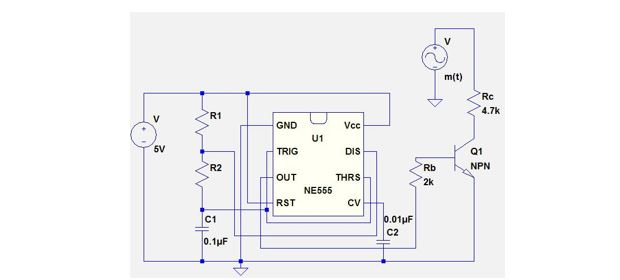
\includegraphics[width = 4in]{./Figures/sampler.jpg}
	    \rule{35em}{0.5pt}
	    \caption{Sampler using 555 Timer Circuit}
    \end{figure}
\end{itemize}
\begin{itemize}
    \item 555 timer is used to generate the switching sequence for the transistor which is operated in its saturation region. 555 timer is used in its astable mode as described above. The duty cycle of the output square wave is set to be much higher than 50\% to generate the sampled impulses at the output. This is in accordance with the Nyquist Sampling Theorem.

    \item The input to the transistor is shown in Figure 2.2.     
    \begin{figure}[htbp]
	    \centering
	    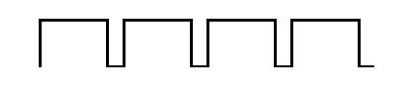
\includegraphics[width = 4in]{./Figures/input.jpg}
	    \rule{35em}{0.5pt}
	    \caption{input to the transistor}
    \end{figure}

    \item The time period of such an astable output is given by the sum of high time and low time. 
        \[T_H=0.7(R_1 + R_2) C_1\] 
        \[T_L=0.7*R_2*C_1\] 
    where T_H and T_L are high and low times, respectively.
\end{itemize}
\begin{itemize}
    \item Design 555 timer in astable mode so that duty cycle of the output waveform is 95\%. Use:
    \[C_1=0.1uF\]

    \item	The baseband signal m(t) is connected in series with the transistor. A dc component is added to m(t) to ensure that it remains positive. Negative values of m(t) cannot keep transistor in saturation mode. When transistor is OFF, m(t) appears at the output and when it is ON output voltage is zero. In this way m(t) is sampled.

    \item Keep the baseband signal amplitude to 2V and dc offset to 3V.

    \item Observe the sampled output on oscilloscope.
    \begin{figure}[htbp]
	    \centering
	    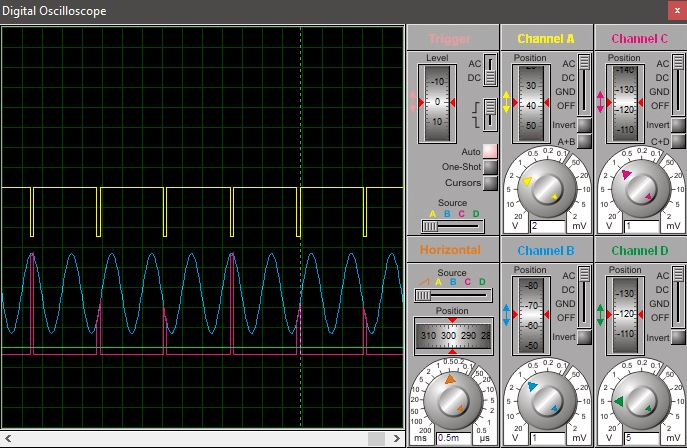
\includegraphics[width = 4in]{./Figures/general-output.jpg}
	    \rule{35em}{0.5pt}
	    \caption{Output of transistor without filter}
    \end{figure}
    
\end{itemize}

 % What to Write 

% Chapter 3

\chapter{Designing of filter} % Write in your own chapter title
\label{Chapter2}
\lhead{Chapter 3. \emph{Designing of filter}} % Write in your own chapter title to set the page header
 \section{Low pass filter design}
 The sampling period in this case will be

    \[T_S=T_H+T_L\]
The sampling period can be changed by changing the time period of the output waveform. Change the sampling time by using different values of resistors keeping the duty cycle to 95\%.


	Finally, you can design a filter to obtain the signal m(t). The filter will be a simple first order RC low pass as shown in Figure 3.1. Choose the cut of frequency of your filter less than the sampling frequency to obtain m(t) at the filter output.
    \[RC < \frac{1}{2} \]

	\begin{figure}[htbp]
	\centering
	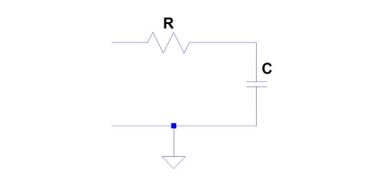
\includegraphics[width = 4in]{./Figures/filter.jpg}
	\rule{35em}{0.5pt}
	\caption{Low pass RC filter}
\end{figure} % What to Write 

%\input{./Chapters/Chapter5} % Experiment 2

%\input{./Chapters/Chapter6} % Results and Discussion

% Chapter 3

\chapter{Circuit Diagram and Calculation} % Write in your own chapter title
\label{Chapter2}
\lhead{Chapter 3. \emph{Circuit Diagram and Calculation}} % Write in your own chapter title to set the page header
 \section{Shematic}
 Below is the shematic of 555 Sampler that is simulated on proteus.
 	\begin{figure}[htbp]
	\centering
	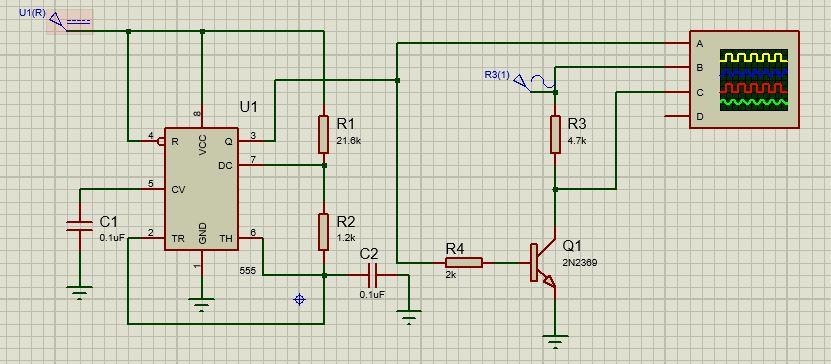
\includegraphics[width = 4in]{./Figures/schematic.jpg}
	\rule{35em}{0.5pt}
	\caption{schematic}
\end{figure}

 \section{calculation}
 \subsection{Different R value combinations at 95\%}
 frequency calculation:
   \[f_s = \frac{1}{T}=\frac{1.44}{(R_1 + 2R_2)C_1} \]
 Duty cycle calculation:
    \[D = \frac{R_2}{R_1+2R_2} \]
High and Low Time
    \[T_H=0.7(R_1 + R_2) C_1\] 
    \[T_L=0.7*R_2*C_1\] 
 \begin{center}
 \begin{tabular}{ |p{3cm}|p{3cm}|p{3cm}|  }
 	\hline
 	\multicolumn{3}{|c|}{Input parameters} \\
 	\hline
 	Capacitance C_1& Value of Resistance R_1 &Value of Resistance R_2\\
 	\hline
 	0.1uF & 3.24$k\Omega$ & 180$\Omega$\\
 	\hline
 \end{tabular}
 \end{center}
  \begin{center}
 \begin{tabular}{ |p{3cm}|p{3cm}|p{3cm}|p{3cm}| }
 	\hline
 	\multicolumn{4}{|c|}{Output parameters} \\
 	\hline
 	Frequency& Time period &High time & Low Time\\
 	\hline
 	4 kHz & 25 millisecond & 23.94 millisecond& 126 millisecond\\
 	\hline
 \end{tabular}
 \end{center}
 	\begin{figure}[htbp]
	\centering
	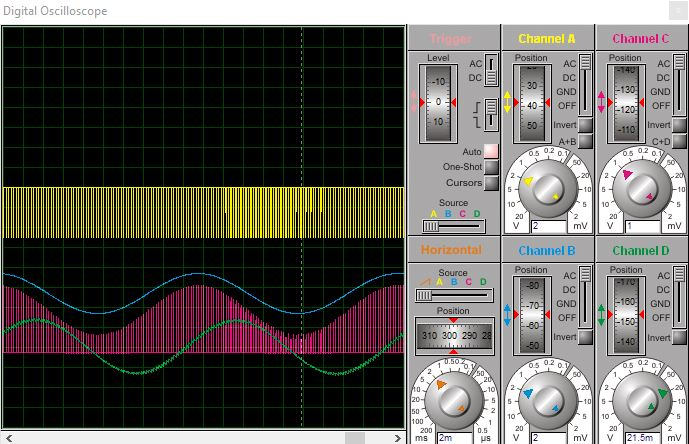
\includegraphics[width = 4in]{./Figures/1.jpg}
	\rule{35em}{0.5pt}
	\caption{schematic}
\end{figure}
	
\begin{center}
 \begin{tabular}{ |p{3cm}|p{3cm}|p{3cm}|  }
 	\hline
 	\multicolumn{3}{|c|}{Input parameters} \\
 	\hline
 	Capacitance C_1& Value of Resistance R_1 &Value of Resistance R_2\\
 	\hline
 	0.1uF & 8.46$k\Omega$ & 470$\Omega$\\
 	\hline
 \end{tabular}
 \end{center}
  \begin{center}
 \begin{tabular}{ |p{3cm}|p{3cm}|p{3cm}|p{3cm}| }
 	\hline
 	\multicolumn{4}{|c|}{Output parameters} \\
 	\hline
 	Frequency& Time period &High time & Low Time\\
 	\hline
 	1531.9 Hz & 65.28 millisecond & 62.51 millisecond& 329 millisecond\\
 	\hline
 \end{tabular}
 \end{center}
 	\begin{figure}[htbp]
	\centering
	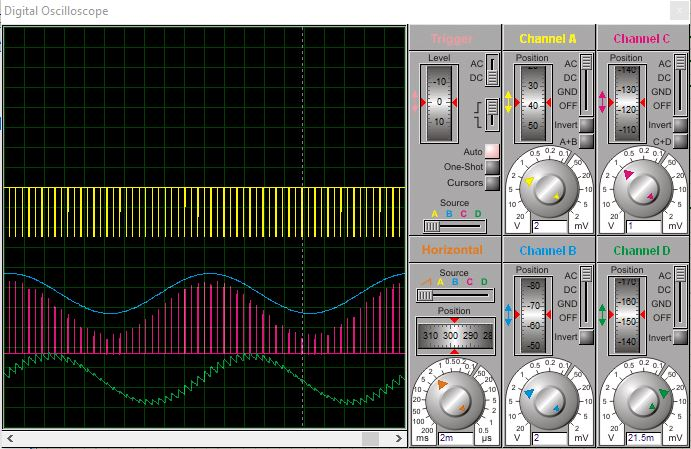
\includegraphics[width = 4in]{./Figures/2.jpg}
	\rule{35em}{0.5pt}
	\caption{schematic}
\end{figure}
\section{Design of filter}
As we know that 
  \[RC < \frac{1}{2} \]
  \begin{figure}[htbp]
	\centering
	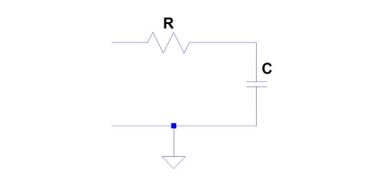
\includegraphics[width = 4in]{./Figures/filter.jpg}
	\rule{35em}{0.5pt}
	\caption{Low pass RC filter}
\end{figure}
\\Value of Resistance R_1 = \underline{3240$\Omega$} 
\\Value of Resistance R_2 = \underline{180$\omega$} 
\\sampling frequency = \underline{4000kHz} 
\\Resistanc value = \underline{8$k\Omega$} 
\\Capacitance = \underline{1uF} 
	\begin{figure}[htbp]
	\centering
	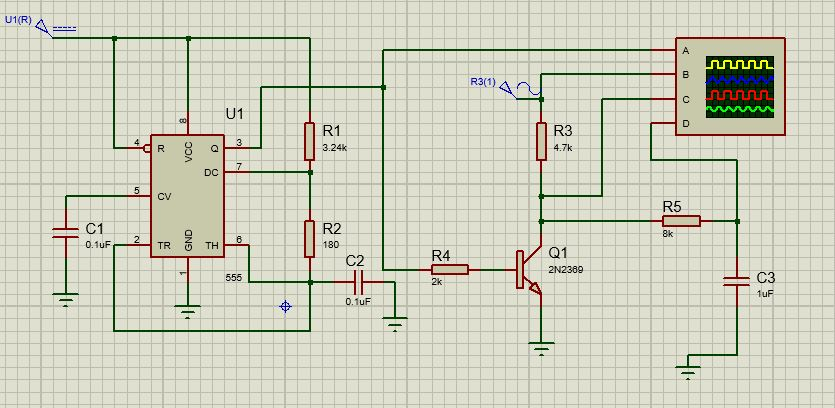
\includegraphics[width = 4in]{./Figures/schematic1.jpg}
	\rule{35em}{0.5pt}
	\caption{sampling at 4000 Hz}
\end{figure}

\\Value of Resistance R_1 = \underline{3240$\Omega$} 
\\Value of Resistance R_2 = \underline{180$\omega$} 
\\sampling frequency = \underline{4000kHz} 
\\Resistanc value = \underline{8$k\Omega$} 
\\Capacitance = \underline{1uF} 
	\begin{figure}[htbp]
	\centering
	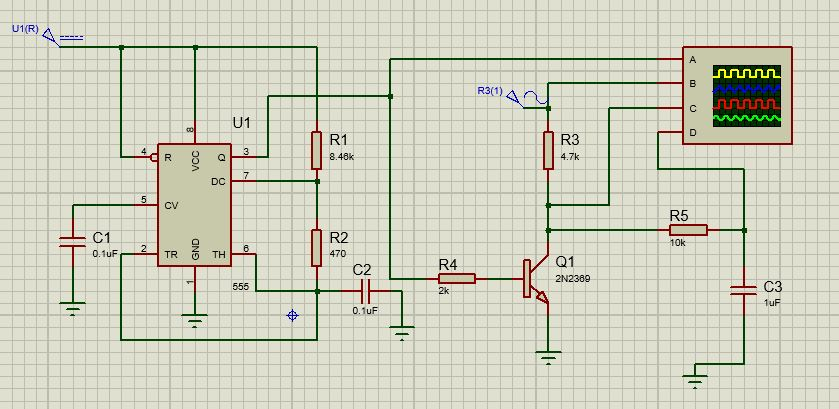
\includegraphics[width = 4in]{./Figures/schematic2.jpg}
	\rule{35em}{0.5pt}
	\caption{sampling at 1531 Hz}
\end{figure} % Conclusion

%% ----------------------------------------------------------------
% Now begin the Appendices, including them as separate files

%\input{./Chapters/AppendixB} % Appendix Title

%\input{./Chapters/AppendixC} % Appendix Title

%% ----------------------------------------------------------------


\end{document}  % The End
%% ----------------------------------------------------------------
